\section{Image Classification}
Machine learning algorithms were defined by \cite{mitchell1997machine} as a computer program that learns from experience E with respect to some class of tasks T, whose performance P improves with experience E. Among the various tasks, classification, especially image classification (along with object recognition) is one of the most common ones. Modern image classification\cite{ioffe2015batch, krizhevsky2012imagenet} and object recognition\cite{taigman2014deepface} is best accomplished with deep CNN. We built a deep convolutional neural network with 16 layers and 1212708 parameters that classifies input images into 4 categories.
\subsection{Training Data}
Most of our training data was retrieved by a web crawler\footnote{See Section \ref{sec:supplementary}} from Microsoft Cognitive Service. Some of the photos were taken manually. The dataset was stratified sampled into a training set and a validation set in respect of a ratio of approximately 3:1. The detailed constitution of the dataset is listed in Table \ref{tab:dataset}.
\begin{table}[htbp]
\centering
\begin{tabular}{c | c c}
\hline
Category & Training & Validation \\
\hline
The Auditorium & 77 & 23\\
The Old Gate & 107 & 40\\
Tsinghua School & 74 & 25\\
The Main Building & 27 & 10\\
\hline
Total & 285 & 98\\
\hline
\end{tabular}
\caption{Constitution of the dataset.}
\label{tab:dataset}
\end{table}
\subsection{Augmentation}
Our neural network takes an input of 150 pixels $\times$ 150 pixels with three channels, therefore all images were first resized to fit the model. All pixels were then applied a mapping to be rescaled from
 $\{n\in\mathbb{N}~|~0\leq n \leq 255\}^3$ to $\{x\in\mathbb{R}~|~0\leq x \leq 1\}^3$. To make up for the limited set of inputs, all images were randomly sheared, zoomed and performed horizontal flips so that the network will not be fed with duplicated inputs.
\subsection{Network}
The neural network we applied is a simplified version of VGG-16\cite{simonyan2014very}. The overall structure of the network is illustrated in Figure \ref{fig:overview}, while layer detail of each component is shown in Figure \ref{fig:model}. In general, the neural network represents a mapping from $\{x\in\mathbb{R}~|~0\leq x \leq 1\}^{3\times150\times150}$ to $\{x\in\mathbb{R}~|~0\leq x \leq 1\}^4$.

\begin{figure}[htbp]
    \centering
    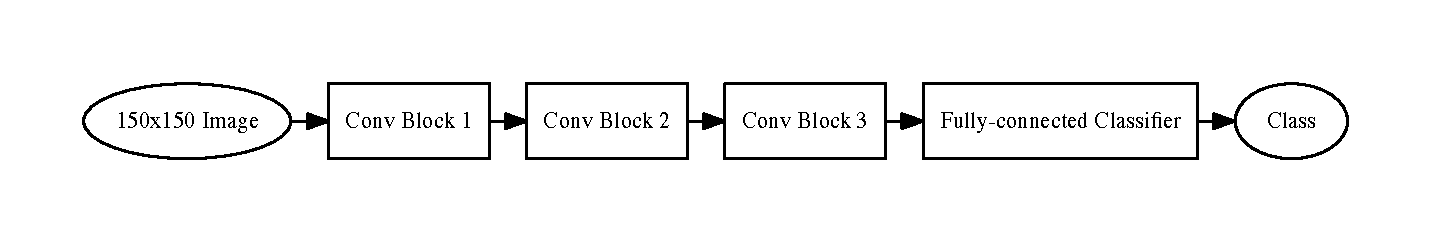
\includegraphics[width=0.9\textwidth]{model}
    \caption{Overview of the neural network.}
    \label{fig:overview}
\end{figure}

\begin{figure}[htbp]
    \begin{subfigure}[b]{0.24\textwidth}
        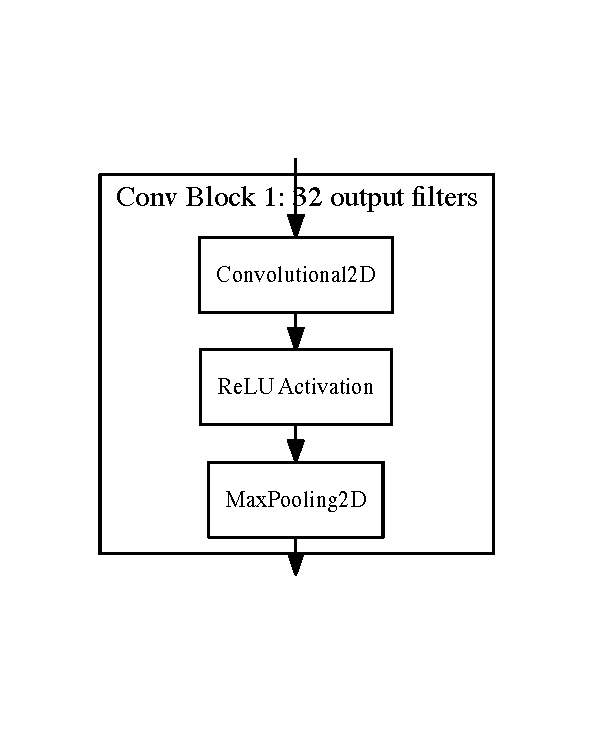
\includegraphics[width=0.95\linewidth]{conv1}
        \caption{Conv Block 1}
        \label{fig:conv1}
    \end{subfigure}
    \begin{subfigure}[b]{0.24\textwidth}
        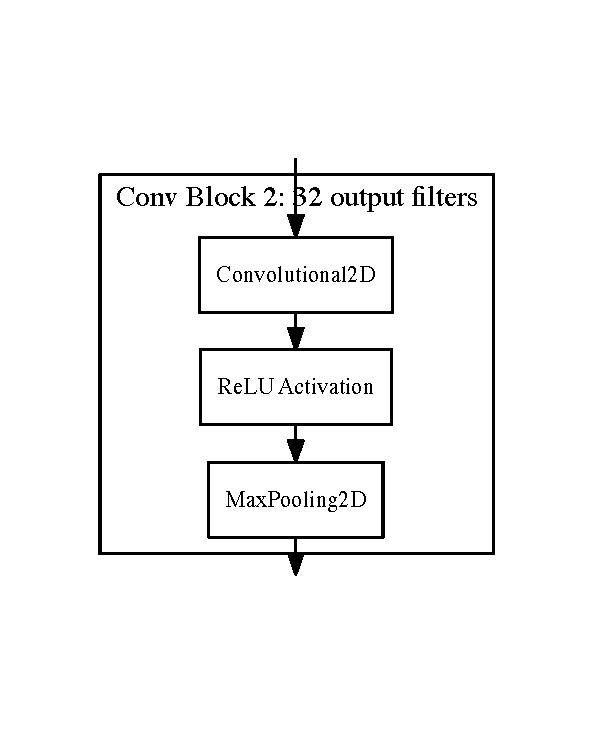
\includegraphics[width=0.95\linewidth]{conv2}
        \caption{Conv Block 2}
        \label{fig:conv2}
    \end{subfigure}
    \begin{subfigure}[b]{0.24\textwidth}
        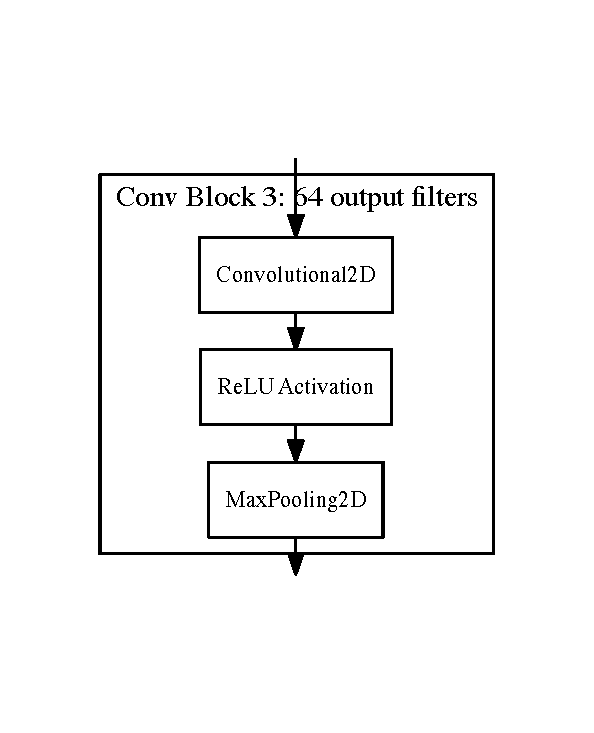
\includegraphics[width=0.95\linewidth]{conv3}
        \caption{Conv Block 3}
        \label{fig:conv3}
    \end{subfigure}
    \begin{subfigure}[b]{0.24\textwidth}
        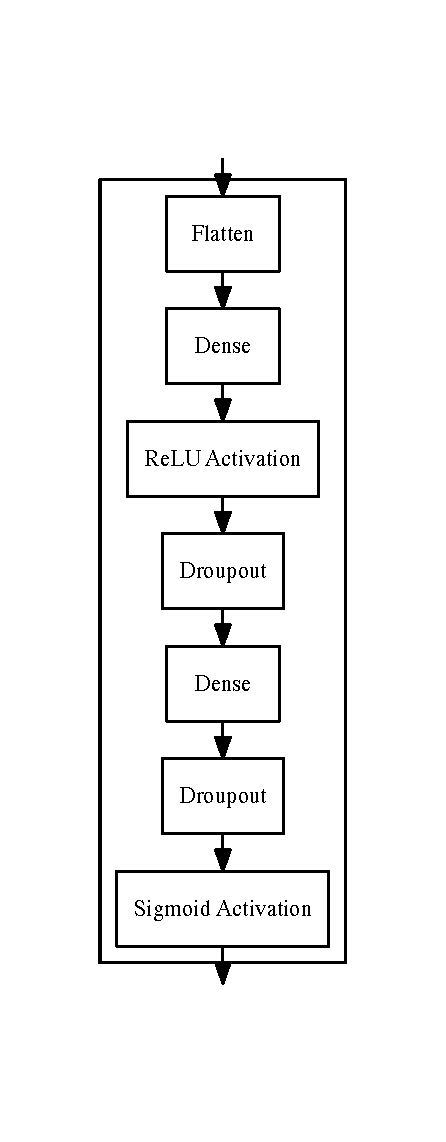
\includegraphics[width=0.95\linewidth]{classifier}
        \caption{Classifier}
        \label{fig:classifier}
    \end{subfigure}
\caption{Detailed model of the neural network.}
\label{fig:model}
\end{figure}

As is shown in Figure \ref{fig:conv1}, \ref{fig:conv2} and \ref{fig:conv3}, the network begins with a cascading of a similar structure: In the first stage, the network performs several convolutions in parallel to produce a set of linear activations. In the second stage, each linear activation is run through a nonlinear activation function, in this case the rectified linear activation function, which is called \emph{the detector stage}. In the third stage, we use a pooling function to modify the output of the layer further\cite{dlbook}. Rectified linear units, or ReLU, uses the activation function
\[
  g(z)=\mathrm{max}\{0,z\}
\]
and the overall activation of a \emph{conv block} would be
\[
  \boldsymbol{h} = g(\boldsymbol{W}^\top \boldsymbol{x} + \boldsymbol{b})\textrm{.}
\]
ReLUs are similar to linear units so they are easy to optimize. \emph{Max pooling}\cite{zhou1988computation} replaces the output of the network at a certain place with the maximum output within its rectangular neighborhood, which helps to make the representation become approximately invariant to small translations of the input\cite{dlbook}.

After all convolution operations, the tensor was then flattened to a column vector, which represents features the net extracted. Then we applied fully-connected \emph{dense} layers, which simply takes the form of
\[
\hat{\boldsymbol{y}} = \boldsymbol{W}^\top \boldsymbol{h} + \boldsymbol{b}\textrm{.}
\]
Typically, as the neural network becomes more complicated, the training error decays but the generalization error increases, causing overfitting\cite{dlbook}, which is illustrated in Figure \ref{fig:overfitting}. In this case the training dataset is too small compared with the deep neural network, so it is prone for the model to overfit. We introduced two layers of \emph{dropout}\cite{srivastava2014dropout} that randomly remove units form the net to avoid overfitting.

\begin{figure}[htbp]
\centering
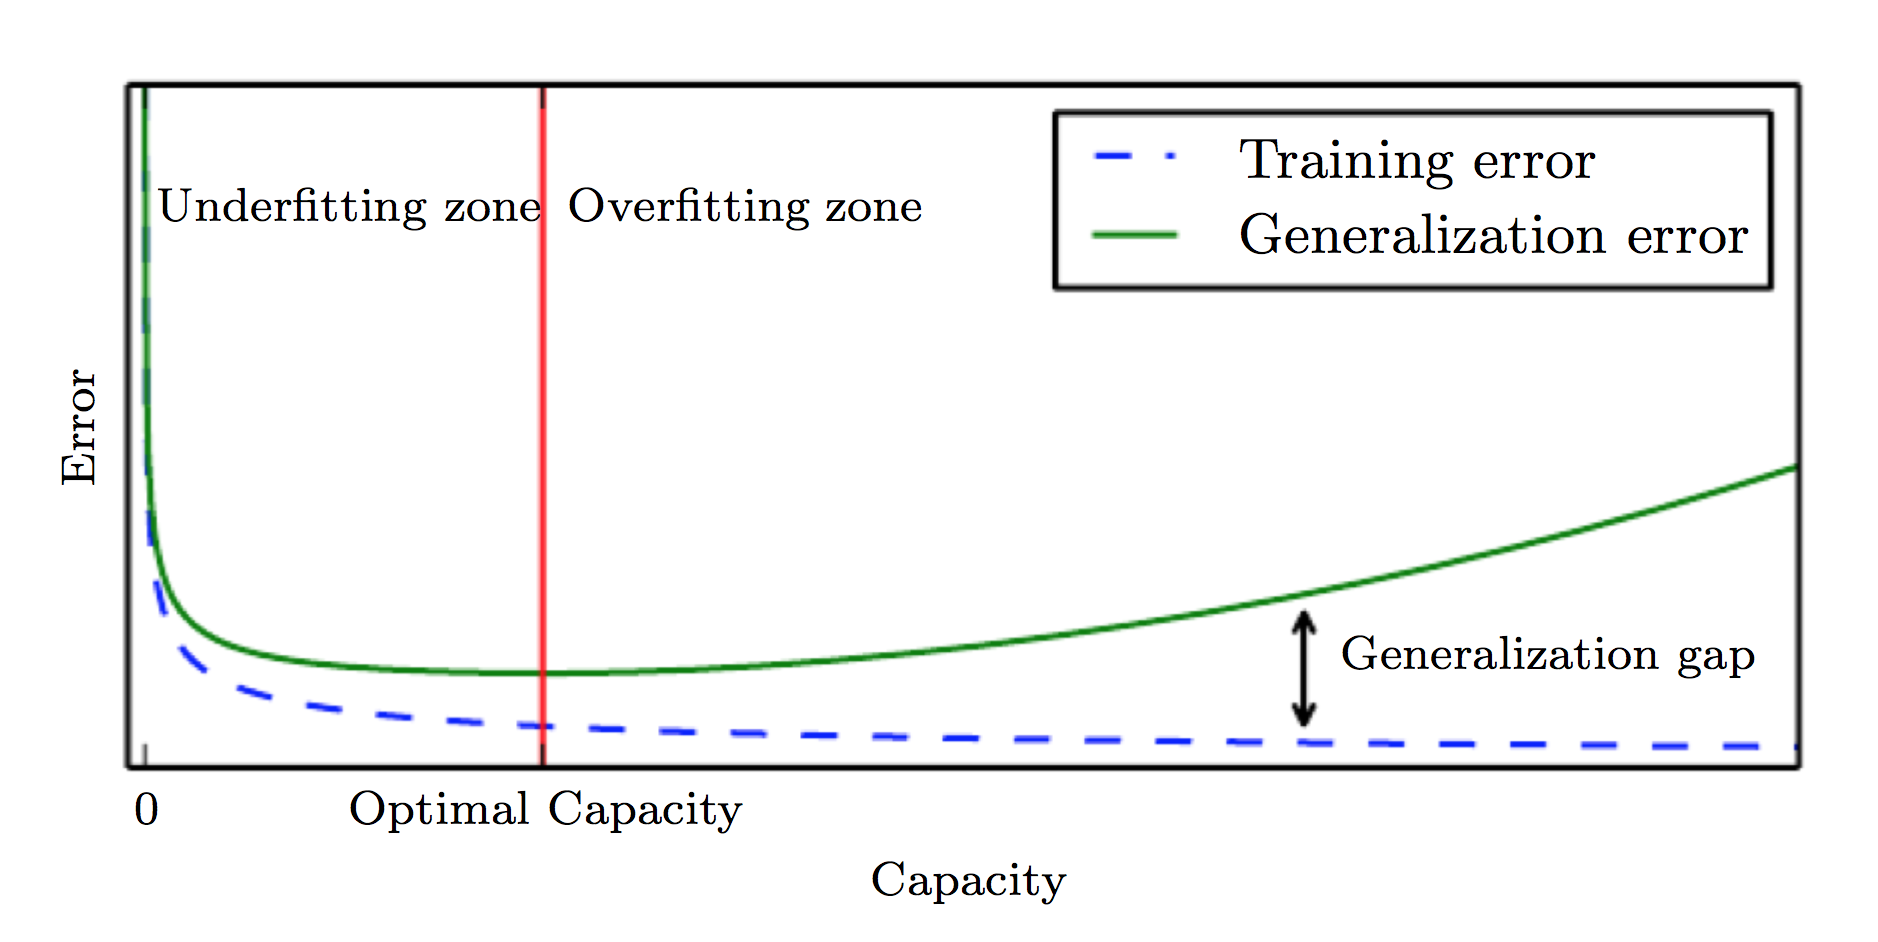
\includegraphics[width=0.8\textwidth]{overfitting}
\caption{Relationship between capacity and error\cite{dlbook}.}
\label{fig:overfitting}
\end{figure}

As the output, we would like to get a probability distribution over all categories, based on which reason a \emph{softmax} output layer was chosen. The final result would be
\[
\hat{y} = \mathrm{P}(y=1~|~\boldsymbol{x})\textrm{.}
\]
The softmax layer first predicts unnormalized log probabilities $z_i = \log\tilde{P}(y=i~|~\boldsymbol{x})$ by
\[
    \boldsymbol{z} = \boldsymbol{W}^\top \boldsymbol{h} + \boldsymbol{b}
\]
and then normalizes it with the softmax function
\[
    \textrm{softmax}(\boldsymbol{z})_i = \frac{\exp(z_i)}{\sum_j\exp{z_j}}\textrm{.}
\]
As we shall see in next subsection, softmax function works well when maximizing the log-likelihood.
\subsection{Cost Function}
Our objective, same as the objective of any other supervised learning, is to maximize the maximum likelihood, which attempts to make the model distribution match the empirical distribution drawn from the training set. Here we use the cross-entropy function
\[
    H_{y'}(y) = -\sum_{i}y_{i}'\log{y_i}
\]
and attempts to minimize it. As can be proved mathematically, minimizing the cross-entropy function defined above is equivalent to minimizing the Kullback-Leibler divergence, which in turn is equivalent to maximizing the maximum likelihood\cite{dlbook}.
\subsection{Training}
The neural network can be depicted as a parametric function $f(\boldsymbol{X};\boldsymbol{\theta})$, and our objective is to optimize the parameter $\boldsymbol{\theta}$ to minimize the cost function. Generally, the cost function and the layers of a typical neural network are all differentiable, which makes neural networks capable of exploiting an algorithms gradient descent. By continuously move from a point $\boldsymbol{x}$ to another point $\boldsymbol{x}'$ where
\[
\boldsymbol{x}' = \boldsymbol{x} - \epsilon\nabla_{\boldsymbol{x}}f(\boldsymbol{x})
\]
our algorithm will eventually get to an approximative minimal or minimum of the cost function. The chain rule of calculus
\[
    \nabla_{\boldsymbol{x}}z = (\frac{\partial{\boldsymbol{y}}} {\partial{\boldsymbol{x}}})^\top\nabla_{\boldsymbol{y}}z
\]
enables the back-propagation algorithm to update every parameter in the neural network to obtain a minimal. It is obvious that the choice of $\epsilon$ is essential because if $\epsilon$ is too large the algorithm may oscillate near a minimal and if too small it will take a long time to converge. In particular we adopted Adam\cite{chilimbi2014project} which is a derivative of the classical stochastic gradient descent algorithms that adopts adaptive momentum that simply put changes $\epsilon$ dynamically to build an efficient and scalable deep learning training system.

After 5,000 iterations, both the training error and the validation error which reflects the generalization error came to a relative low rate. The process of how the training error and the validation error evolves through iterations is plotted in Figure \ref{fig:training}.
\begin{figure}[htbp]
    \centering
    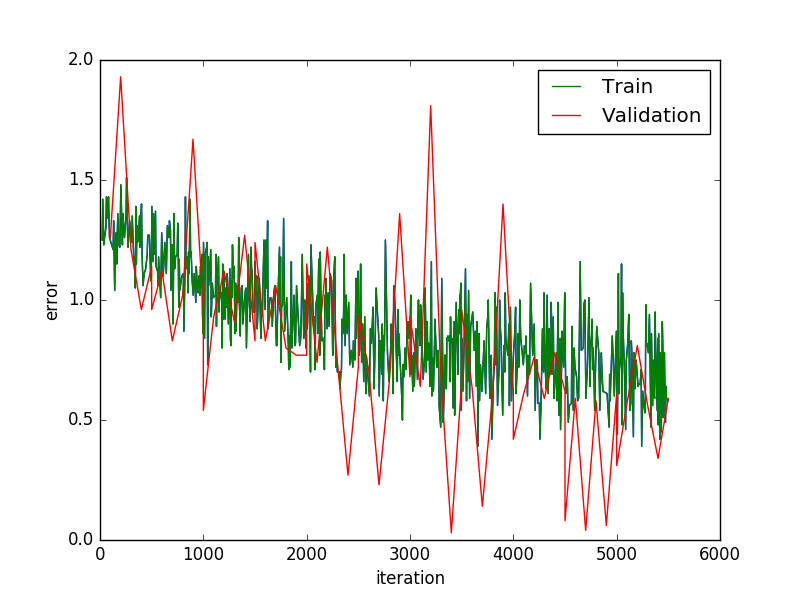
\includegraphics[width=0.7\textwidth]{training}
    \caption{The evolvement of training error and validation error.}
    \label{fig:training}
\end{figure}
\subsection{Evaluation}
The trained model correctly predicts 80 percent of the samples in the randomly sampled validation set and performed satisfyingly in real-world tests in our live demonstration.

After training, the error on the training set and that on the validation set did not seem to converge at that time but in order to avoid overfitting the training was terminated. But there exists possibility that the training error and the generalization error could be further lowered.

Compared with other typical applications of deep neural network, our dataset is definitely too limited that can not utilize the full potential of deep neural networks. Other approaches, like support vector machine\cite{boser1992training} or traditional computer vision methods like manual feature extraction might perform better or equally given the same task and training set.
